\documentclass[10pt]{article}
\usepackage[a4paper,margin=18mm]{geometry}
\usepackage{amsmath,amssymb,booktabs,array,enumitem}
\usepackage[T1]{fontenc}\usepackage{lmodern}
\usepackage{tikz}\usetikzlibrary{shapes.gates.logic.US,positioning,arrows.meta,patterns,calc}
\usepackage[hidelinks]{hyperref}
\setlength{\parindent}{0pt}\setlength{\parskip}{4pt}
\setlength{\emergencystretch}{2em}
\newcommand{\VDD}{V_{DD}}
\newcommand{\mos}[4]{\begin{scope}[shift={(#1,#2)}]
\draw (0,.24)--(0,-.24);\draw (0,.20)--(.25,.20)--(.25,.5);
\draw (0,-.20)--(.25,-.20)--(.25,-.5);\draw (-.16,.23)--(-.16,-.23);
\ifnum#4=1\draw (-.26,0) circle (.06);\draw (-.75,0)--(-.32,0);\else\draw (-.75,0)--(-.16,0);\fi
\node[anchor=east,font=\scriptsize] at (-.76,0) {$#3$};\end{scope}}
\newcommand{\ground}[2]{\draw (#1,#2)--(#1,{#2-.12});\draw ({#1-.17},{#2-.12})--({#1+.17},{#2-.12});\draw ({#1-.11},{#2-.20})--({#1+.11},{#2-.20});}
\newcommand{\rail}[3]{\draw (#1,#2)--(#1,{#2+.14});\node[above,font=\scriptsize] at (#1,{#2+.14}) {$#3$};}

\newcommand{\hmos}[4]{\begin{scope}[shift={(#1,#2)}]
\draw(-.24,0)--(.24,0);\draw(-.2,0)--(-.2,-.25)--(-.5,-.25);\draw(.2,0)--(.2,-.25)--(.5,-.25);
\draw(-.23,.16)--(.23,.16);
\ifnum#4=1\draw(0,.26)circle(.06);\draw(0,.32)--(0,.75);\else\draw(0,.16)--(0,.75);\fi
\node[below,font=\scriptsize]at(0,-.32){#3};\end{scope}}
\newcommand{\mosvt}[5]{\mos{#1}{#2}{#3}{#4}\ifnum#5=1\draw[line width=1.1pt]({#1-.16},{#2-.23})--({#1-.16},{#2+.23});\fi}\begin{document}
\begin{center}{\large\bfseries EE3032 Introduction to VLSI -- Midterm}\\Fall 2011\end{center}
\textbf{1. (20 points)} Complete the following problems.
\begin{enumerate}[label=(\alph*),leftmargin=7mm,itemsep=2pt]
\item The layer density rule should be met when you design a nano-scale IC. Why? (2 points)
\item What is the antenna effect? (2 points)
\item Draw a CMOS transistor-level schematic realizing $f=\overline{xy+(u+v)w}$. (4 points)
\item List four properties of static CMOS logic. (4 points)
\item Draw a CMOS inverter and label the drain and source of its PMOS and NMOS. (2 points)
\item List the three major components of load capacitance of a CMOS logic gate in a CMOS circuit. (3 points)
\item How do you size the N and P MOS of an inverter such that its output voltage is $V_{DD}/2$ when its input is $V_{DD}/2$? (3 points)
\end{enumerate}
\textbf{2. (20 points)} An inverter with output load $C_L$, operated at frequency $f$ under supply $V_{DD}$, has switching power $fC_LV_{DD}^2$. If input $t_r=t_f=\tau$ is applied to an inverter with $\beta_n=\beta_p=\beta$, its short-circuit power can be estimated by the printed formula $P_{sc}=k\beta(V_{DD}-V_t)^3\tau f$, where $k$ is a constant. Also $t_r=C_L/(\beta_pV_{DD})$ and $t_f=C_L/(\beta_nV_{DD})$.
\begin{enumerate}[label=(\alph*),leftmargin=7mm]
\item Figure 1 depicts an inverter chain driving $C_L$. Assume $\mu_n=2\mu_p$. A $W/L$ PMOS or NMOS has gate capacitance $C_g$, and a $W/L$ NMOS has $\beta_n=\beta$. Drain/wire parasitics are neglected. A unit delay is $\tau_0=C_g/(\beta V_{DD})$ ns. Calculate the dynamic power (switching and short-circuit) of the chain when the shown waveform is applied to its input at switching frequency $f$. (10 points)
\item The minimum-size inverter has $W/L$ NMOS and $W/L$ PMOS, with total input capacitance $C_g$; its delay driving $C_g$ is $t_d$. For brevity, assume $e=2$ and neglect drain/wire capacitance. Design a buffer chain driving $C_L=64C_g$ with minimized delay. Draw the chain, label transistor sizes, and explain. (10 points)
\end{enumerate}
\begin{center}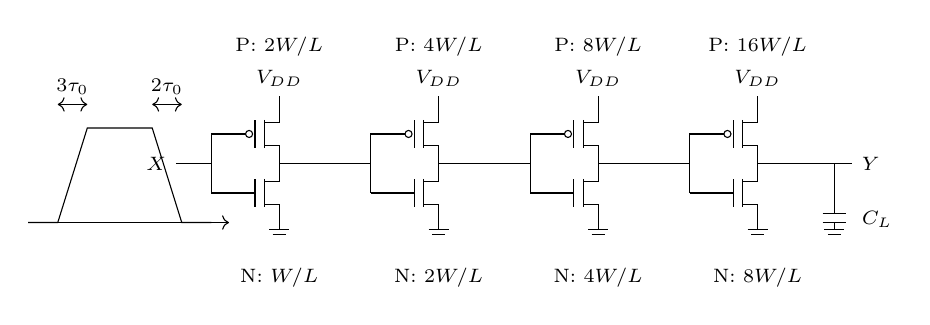
\begin{tikzpicture}[x=.75cm,y=.75cm,font=\scriptsize]
\draw[->](-1,0)--(2.4,0);\draw(-1,0)--(-.5,0)--(0,1.6)--(1.1,1.6)--(1.6,0)--(2.1,0);\draw[<->](-.5,2)--(0,2)node[midway,above]{$3\tau_0$};\draw[<->](1.1,2)--(1.6,2)node[midway,above]{$2\tau_0$};
\mos{3.0}{1.5}{}{1}\mos{3.0}{.5}{}{0}\rail{3.25}{2}{V_{DD}}\ground{3.25}{0}\draw(2.1,.5)--(2.1,1.5)--(2.25,1.5);\draw(2.1,.5)--(2.25,.5);
\node[above]at(3.25,2.65){P: $2W/L$};\node[below]at(3.25,-.6){N: $W/L$};
\draw(1.5,1)--(2.1,1)node[pos=0,left]{$X$};
\mos{5.7}{1.5}{}{1}\mos{5.7}{.5}{}{0}\rail{5.95}{2}{V_{DD}}\ground{5.95}{0}\draw(4.8,.5)--(4.8,1.5)--(4.95,1.5);\draw(4.8,.5)--(4.95,.5);
\node[above]at(5.95,2.65){P: $4W/L$};\node[below]at(5.95,-.6){N: $2W/L$};
\draw(3.25,1)--(4.8,1);
\mos{8.4}{1.5}{}{1}\mos{8.4}{.5}{}{0}\rail{8.65}{2}{V_{DD}}\ground{8.65}{0}\draw(7.5,.5)--(7.5,1.5)--(7.65,1.5);\draw(7.5,.5)--(7.65,.5);
\node[above]at(8.65,2.65){P: $8W/L$};\node[below]at(8.65,-.6){N: $4W/L$};
\draw(5.95,1)--(7.5,1);
\mos{11.100000000000001}{1.5}{}{1}\mos{11.100000000000001}{.5}{}{0}\rail{11.350000000000001}{2}{V_{DD}}\ground{11.350000000000001}{0}\draw(10.200000000000001,.5)--(10.200000000000001,1.5)--(10.350000000000001,1.5);\draw(10.200000000000001,.5)--(10.350000000000001,.5);
\node[above]at(11.350000000000001,2.65){P: $16W/L$};\node[below]at(11.350000000000001,-.6){N: $8W/L$};
\draw(8.650000000000002,1)--(10.200000000000001,1);
\draw(11.350000000000001,1)--(12.950000000000001,1)node[right]{$Y$};\draw(12.650000000000002,1)--(12.650000000000002,.15);\draw(12.450000000000001,.15)--(12.850000000000001,.15);\draw(12.450000000000001,0)--(12.850000000000001,0);\ground{12.650000000000002}{0}\node[right]at(12.950000000000001,.05){$C_L$};
\end{tikzpicture}\\Figure 1: Inverter chain; PMOS/NMOS widths are 2/1, 4/2, 8/4, 16/8 times W.\end{center}
\newpage
\textbf{3. (20 points)} Figure 2(a) depicts a CMOS logic circuit. An inverter has delay 1 unit, with $W_p/L_p=2\,\mu\mathrm m/0.18\,\mu\mathrm m$, $W_n/L_n=1\,\mu\mathrm m/0.18\,\mu\mathrm m$, and input capacitance $C_g$. All transistors in the other gates have the corresponding same sizes. Functional inputs are $\{I_0I_1I_2I_3\}=\{0100,0011,1100,1011\}$, periodically applied in sequence at frequency $f$ under supply $V_{DD}$.
\begin{enumerate}[label=(\alph*),leftmargin=7mm]
\item A dual-$V_T$ process can implement the circuit. Draw its transistor-level schematic using the symbols in Figure 2(b), such that leakage power is minimal without sacrificing speed. (10 points)
\item Assume all logic gates in Figure 2(a) have the same delay. Does the circuit exhibit glitches? Explain. (10 points)
\end{enumerate}
\begin{center}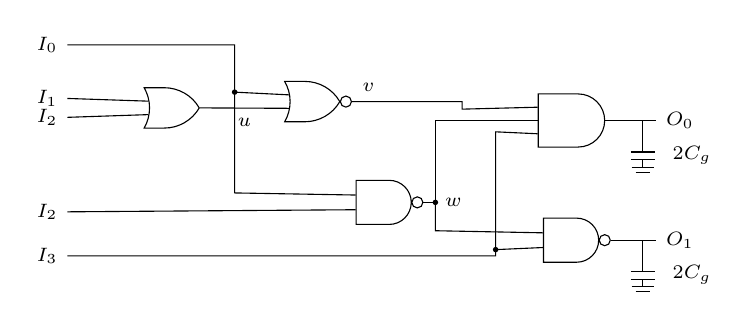
\begin{tikzpicture}[x=.85cm,y=.8cm,font=\scriptsize]
\node[or gate US,draw,logic gate inputs=nn,minimum width=.7cm](u)at(1.2,3){};\node[nor gate US,draw,logic gate inputs=nn,minimum width=.7cm](v)at(3.3,3.1){};\node[nand gate US,draw,logic gate inputs=nn,minimum width=.7cm](w)at(4.4,1.5){};\node[and gate US,draw,logic gate inputs=nnn,minimum width=.7cm](a)at(7.2,2.8){};\node[nand gate US,draw,logic gate inputs=nn,minimum width=.7cm](b)at(7.2,.9){};
\draw(u.input 1)--(-.3,3.15)node[left]{$I_1$};\draw(u.input 2)--(-.3,2.85)node[left]{$I_2$};\draw(u.output)--(v.input 2)node[midway,below]{$u$};\draw(-.3,4)node[left]{$I_0$}--(2.2,4)--(2.2,3.25)--(v.input 1);\draw(2.2,3.25)--(2.2,1.65)--(w.input 1);\fill(2.2,3.25)circle(1pt);\draw(-.3,1.35)node[left]{$I_2$}--(w.input 2);
\draw(v.output)--(5.6,3.1)--(5.6,2.98)--(a.input 1);\node[above]at(4.2,3.1){$v$};\draw(w.output)--(5.2,1.5)--(5.2,2.8)--(a.input 2);\draw(5.2,1.5)--(5.2,1.05)--(b.input 1);\fill(5.2,1.5)circle(1pt);\node[right]at(5.2,1.5){$w$};\draw(-.3,.65)node[left]{$I_3$}--(6.1,.65)--(6.1,.75)--(b.input 2);\draw(6.1,.75)--(6.1,2.62)--(a.input 3);\fill(6.1,.75)circle(1pt);
\draw(a.output)--(8.5,2.8)node[right]{$O_0$};\draw(b.output)--(8.5,.9)node[right]{$O_1$};\foreach\y in {2.8,.9}{\draw(8.3,\y)--(8.3,\y-.5);\draw(8.12,\y-.5)--(8.48,\y-.5);\draw(8.12,\y-.62)--(8.48,\y-.62);\ground{8.3}{\y-.62}\node[right]at(8.6,\y-.55){$2C_g$};}\end{tikzpicture}\\(a) CMOS circuit\\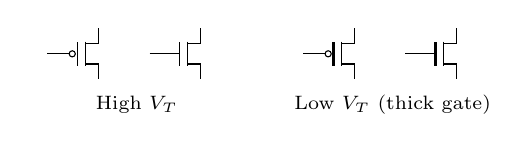
\begin{tikzpicture}[font=\scriptsize,scale=.65]\mosvt{0}{0}{}{1}{0}\mosvt{2}{0}{}{0}{0}\node at(1,-1){High $V_T$};\mosvt{5}{0}{}{1}{1}\mosvt{7}{0}{}{0}{1}\node at(6,-1){Low $V_T$ (thick gate)};\end{tikzpicture}\\(b) High- and low-$V_T$ symbols\\Figure 2.\end{center}
\textbf{4. (20 points)} Figure 3 shows a pass-transistor logic circuit. Assume $V_{DD}=1.8$ V and NMOS threshold voltage $0.4$ V.
\begin{enumerate}[label=(\alph*),leftmargin=7mm]
\item Draw Y and Z waveforms for the shown X input, label minimum and maximum voltages, and explain. (10 points)
\item Neglect body effect and apply the same input. (i) Identify which of m1--m6 can operate in saturation and linear regions; explain. (5 points) (ii) Identify which can operate only in the linear region; explain. (5 points)
\end{enumerate}
\begin{center}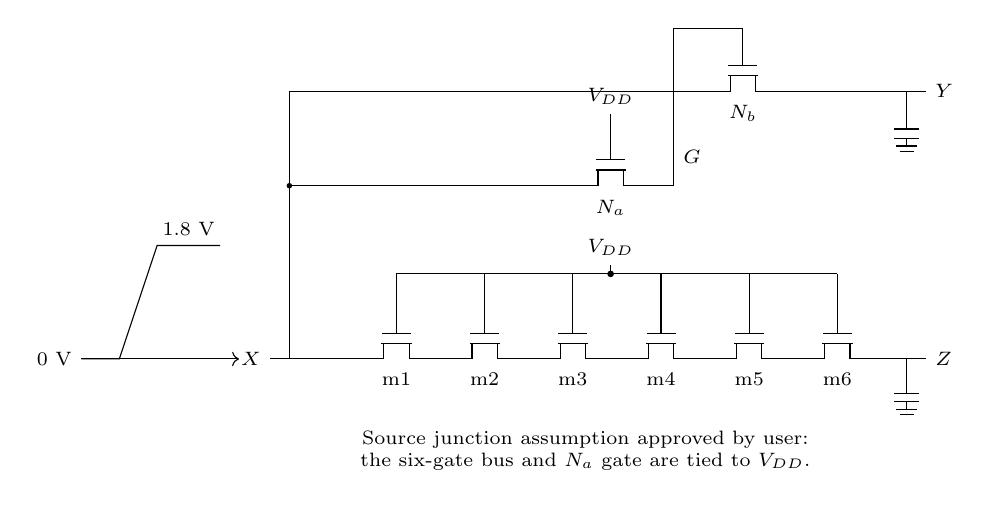
\begin{tikzpicture}[x=.8cm,y=.8cm,font=\scriptsize]
\draw[->](-4,0)--(-1.5,0);\draw(-4,0)--(-3.4,0)--(-2.8,1.8)--(-1.8,1.8);\node[left]at(-4,0){0 V};\node[above]at(-2.3,1.8){1.8 V};\draw(-1,0)node[left]{$X$}--(.3,0);
\hmos{1.0}{.25}{m1}{0}
\draw(.3,0)--(0.5,0);
\draw(1.0,1)--(1.0,1.35);
\hmos{2.4}{.25}{m2}{0}
\draw(1.5,0)--(1.9,0);
\draw(2.4,1)--(2.4,1.35);
\hmos{3.8}{.25}{m3}{0}
\draw(2.9,0)--(3.3,0);
\draw(3.8,1)--(3.8,1.35);
\hmos{5.199999999999999}{.25}{m4}{0}
\draw(4.299999999999999,0)--(4.699999999999999,0);
\draw(5.199999999999999,1)--(5.199999999999999,1.35);
\hmos{6.6}{.25}{m5}{0}
\draw(5.699999999999999,0)--(6.1,0);
\draw(6.6,1)--(6.6,1.35);
\hmos{8.0}{.25}{m6}{0}
\draw(7.1,0)--(7.5,0);
\draw(8.0,1)--(8.0,1.35);
\draw(1,1.35)--(8,1.35);\rail{4.4}{1.35}{V_{DD}}\fill(4.4,1.35)circle(1.2pt);\draw(8.5,0)--(9.4,0)node[right]{$Z$};\draw(9.1,0)--(9.1,-.55);\draw(8.9,-.55)--(9.3,-.55);\draw(8.9,-.68)--(9.3,-.68);\ground{9.1}{-.68}
\hmos{4.4}{3}{$N_a$}{0}\hmos{6.5}{4.5}{$N_b$}{0}\draw(-.7,0)--(-.7,2.75)--(3.9,2.75);\draw(-.7,2.75)--(-.7,4.25)--(6,4.25);\fill(-.7,2.75)circle(1pt);\rail{4.4}{3.75}{V_{DD}}\draw(4.9,2.75)--(5.4,2.75)--(5.4,5.25)--(6.5,5.25);\node[right]at(5.4,3.2){$G$};\draw(7,4.25)--(9.4,4.25)node[right]{$Y$};\draw(9.1,4.25)--(9.1,3.65);\draw(8.9,3.65)--(9.3,3.65);\draw(8.9,3.5)--(9.3,3.5);\ground{9.1}{3.5}
\node[align=center]at(4,-1.45){Source junction assumption approved by user:\\the six-gate bus and $N_a$ gate are tied to $V_{DD}$.};\end{tikzpicture}\\Figure 3: Pass-transistor circuit. $N_a,N_b,G$ are added identification labels.\end{center}
\newpage
\textbf{5. (20 points)} Figure 4 depicts an interconnection RC model and different transmission-gate configurations.
\begin{enumerate}[label=(\alph*),leftmargin=7mm]
\item An interconnection is modeled as distributed RC; the delay of an $x\,\mu$m interconnection is estimated as $kx^2$, with constant $k$. What approach reduces interconnection delay? Explain. (5 points)
\item The delay of two cascaded TGs in Figure 4(b) is 9 ns. A buffer driving two TGs / one TG has delay 2 ns / 1 ns, respectively, as shown in (c)/(d). (i) What is the delay of five TGs in (e)? (5 points) (ii) Insert the smallest number of buffers so delay is smaller than 30 ns; draw the circuit and calculate delay. (5 points) (iii) Insert buffers to minimize delay; draw the circuit and calculate delay. (5 points)
\end{enumerate}
\begin{center}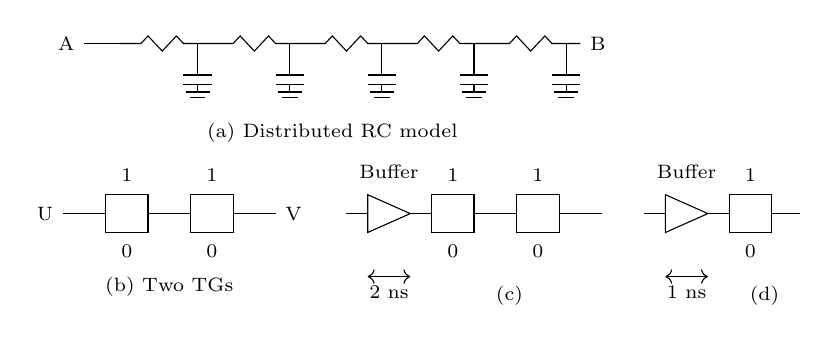
\begin{tikzpicture}[x=.9cm,y=.8cm,font=\scriptsize]
\draw(0,3)node[left]{A}--(.5,3);\foreach\x in {.5,1.8,3.1,4.4,5.7}{\draw(\x,3)--(\x+.3,3)--(\x+.4,3.12)--(\x+.6,2.88)--(\x+.8,3.12)--(\x+.9,3)--(\x+1.3,3);\draw(\x+1.1,3)--(\x+1.1,2.5);\draw(\x+.9,2.5)--(\x+1.3,2.5);\draw(\x+.9,2.35)--(\x+1.3,2.35);\ground{\x+1.1}{2.35}}\node[right]at(7,3){B};\node[below]at(3.5,1.9){(a) Distributed RC model};
\begin{scope}[shift={(0,.3)}]\draw(-.3,0)node[left]{U}--(.3,0);\foreach\x in {.3,1.5}{\draw(\x,-.3)rectangle(\x+.6,.3);\node[above]at(\x+.3,.35){1};\node[below]at(\x+.3,-.35){0};\draw(\x+.6,0)--(\x+1.2,0);} \node[right]at(2.7,0){V};\node[below]at(1.2,-.85){(b) Two TGs};\end{scope}
\begin{scope}[shift={(4,.3)}]\draw(-.3,0)--(0,0);\draw(0,-.3)--(0,.3)--(.6,0)--cycle;\node[above]at(.3,.4){Buffer};\draw(.6,0)--(.9,0);\foreach\x in {.9,2.1}{\draw(\x,-.3)rectangle(\x+.6,.3);\node[above]at(\x+.3,.35){1};\node[below]at(\x+.3,-.35){0};\draw(\x+.6,0)--(\x+1.2,0);} \draw[<->](0,-1)--(.6,-1)node[midway,below]{2 ns};\node[below]at(2,-1){(c)};\end{scope}
\begin{scope}[shift={(8.2,.3)}]\draw(-.3,0)--(0,0);\draw(0,-.3)--(0,.3)--(.6,0)--cycle;\node[above]at(.3,.4){Buffer};\draw(.6,0)--(.9,0);\draw(.9,-.3)rectangle(1.5,.3);\draw(1.5,0)--(1.9,0);\node[above]at(1.2,.35){1};\node[below]at(1.2,-.35){0};\draw[<->](0,-1)--(.6,-1)node[midway,below]{1 ns};\node[below]at(1.4,-1){(d)};\end{scope}\end{tikzpicture}
\begin{tikzpicture}[x=.95cm,y=.8cm,font=\scriptsize]
\draw(-.8,0)node[left]{$X$}--(0,0);
\draw(0,0)--(0.35,0);\draw(0.35,-.3)rectangle(0.85,.3);\node[above]at(0.6,.35){1};\node[below]at(0.6,-.35){0};\draw(0.85,0)--(1.2,0);
\draw(1.2,0)--(1.5499999999999998,0);\draw(1.5499999999999998,-.3)rectangle(2.05,.3);\node[above]at(1.7999999999999998,.35){1};\node[below]at(1.7999999999999998,-.35){0};\draw(2.05,0)--(2.4,0);
\draw(2.4,0)--(2.75,0);\draw(2.75,-.3)rectangle(3.25,.3);\node[above]at(3.0,.35){1};\node[below]at(3.0,-.35){0};\draw(3.25,0)--(3.5999999999999996,0);
\draw(3.5999999999999996,0)--(3.9499999999999997,0);\draw(3.9499999999999997,-.3)rectangle(4.449999999999999,.3);\node[above]at(4.199999999999999,.35){1};\node[below]at(4.199999999999999,-.35){0};\draw(4.449999999999999,0)--(4.8,0);
\draw(4.8,0)--(5.1499999999999995,0);\draw(5.1499999999999995,-.3)rectangle(5.6499999999999995,.3);\node[above]at(5.3999999999999995,.35){1};\node[below]at(5.3999999999999995,-.35){0};\draw(5.6499999999999995,0)--(6.0,0);
\draw(6.0,0)--(6.6,0)node[right]{$Y$};
\end{tikzpicture}\\(e) Five cascaded TGs.\\Figure 4: (a) Wire RC model, (b) two TGs, (c)/(d) buffered TGs, (e) five TGs.\end{center}
\textbf{6. (10 points)} Figure 5 depicts a CMOS inverter process cross section. (a) Draw a circuit model of latchup. (5 points) (b) Explain latchup using the model in (a). (5 points)
\begin{center}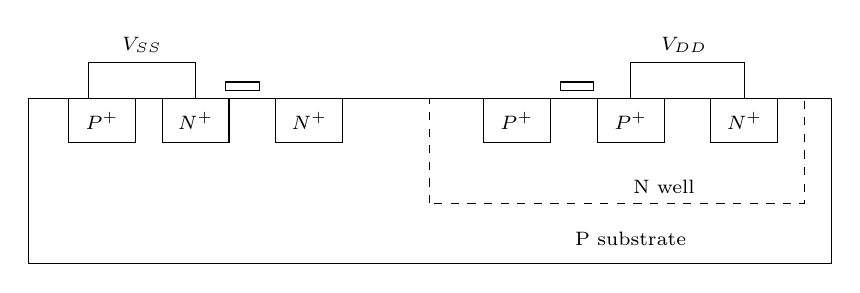
\begin{tikzpicture}[x=.85cm,y=.7cm,font=\scriptsize]
\draw(0,0)rectangle(12,3);\node at(9,.45){P substrate};\draw[dashed](6,1.1)--(6,3)--(11.6,3)--(11.6,1.1)--cycle;\node at(9.5,1.4){N well};\foreach\x/\t in {.6/P^+,2/N^+,3.7/N^+,6.8/P^+,8.5/P^+,10.2/N^+}{\draw(\x,2.2)rectangle(\x+1,3);\node at(\x+.5,2.6){$\t$};}\draw(2.95,3.15)rectangle(3.45,3.3);\draw(7.95,3.15)rectangle(8.45,3.3);\draw(.9,3)--(.9,3.65)--(2.5,3.65)--(2.5,3);\node[above]at(1.7,3.65){$V_{SS}$};\draw(9,3)--(9,3.65)--(10.7,3.65)--(10.7,3);\node[above]at(9.8,3.65){$V_{DD}$};\end{tikzpicture}\\Figure 5: Process cross-section view of a CMOS inverter.\end{center}
\small Archive note: Six source photograph panels cover the three-page dated Fall 2011 paper. The reconstruction retains their visible question text and circuit connections. Printed question totals sum to 110 points; all original point labels are retained. The user approved the faint VDD-bus junction reconstruction in Figure 3 with this explicit assumption.\end{document}
